\documentclass{article}                                                                           %basic LaTeX document type

\usepackage[margin=1.3in]{geometry}                                                     %set size of all margins
%\usepackage[left=1.3in, top=1in, right=1in, bottom=1in]{geometry}         %can set margin sizes which are not the same in this way

%\linespread{2}                                                                                         %option 1 for making text double-spaced
\usepackage{setspace}                                                                             %option 2 for making text double-spaced
\doublespacing                                                                                         %set double space

\usepackage{indentfirst}                                                                          %makes first paragraph of section indented (non-first are by default)
\setlength{\parindent}{25pt}                                                                     %set size of indentation (15pt is default)

\renewcommand\thesection{\Roman{section}}                                         %set capital Roman numeral section headings
\renewcommand\thesubsection{\thesection.\Alph{subsection}}                   %set capital Aramaic letters subsection headings
\renewcommand\thesubsubsection{\thesubsection.\arabic{subsubsection}} %set capital Arabic numbers subsubsection headings

\renewcommand*\thetable{\Roman{table}}                                              %set capital Roman numeral table numeration

\usepackage[explicit]{titlesec}                                                                  %package needed for next lines
\titleformat{\section}{\bfseries}{\thesection.}{1em}{\MakeUppercase{#1}}  %makes section headings bold and upper case characters
\titleformat{\subsection}{\bfseries}{\thesubsection.}{1em}{#1}                   %makes subsection headings bold
\titleformat{\subsubsection}{\itshape}{\thesubsubsection.}{1em}{#1}          %makes subsubsection headings in italics

\usepackage{lastpage}                                                                             %package which returns number of last page (same as number of pages)
\usepackage[figure,table]{totalcount}                                                        %package which counts the number of tables and/or figures

\usepackage{amsmath}                                                                            %enable `align' equation types

\renewcommand{\thefootnote}{\alph{footnote}}                                        %sets labeling of footnotes
\usepackage[]{footmisc}                                                                          %enables double spaced footnotes
  \renewcommand{\footnotelayout}{\doublespacing}                                  %double spacing of footnotes

%%% If you desire to place footnotes at the end of the document, uncomment these four lines and the two related near the end of this file
%\usepackage{endnotes}                                                                          %enables endnote page
%  \let\footnote=\endnote                                                                         %sets footnotes to endnotes
%  \renewcommand*{\theendnote}{\alph{endnote}}                                   %labels endnotes alphabetically
%  \renewcommand{\notesname}{Footnotes}                                            %renames endnotes title to footnotes

\usepackage{graphicx}                                                                             %enable figures
\usepackage{multirow}                                                                             %enable `multirow' capability in tables

\usepackage{caption}                                                                              %enables subfigures
\usepackage[labelformat=simple]{subcaption}                                           %enables subfigure captions 
\captionsetup[table]{labelsep=newline,name=TABLE}                                 %sets table caption formatting options to meet NSE requirements
\captionsetup[figure]{name=Fig.,labelsep=period}                                     %sets figure caption options to meet NSE requirements
\renewcommand*\thesubfigure{(\alph{subfigure})}                                    %enables proper labeling of subfigures

\usepackage[colorlinks=true, allcolors=blue]{hyperref}                               %reference and citation hyperlinking linking

\usepackage{subfloat}
\usepackage{cite}
\usepackage{lineno, blindtext}

\DeclareMathOperator{\diff}{d}                                                                %can define operators to use in math mode, example in Eq. 2
\DeclareMathOperator{\erf}{erf}

\begin{document}

%Define fields for \maketitle

\title{Analysis of Using a Nuclear Fuel Cycle Simulator to Model a Nuclear Renewable Hybrid Energy System} %title of paper

\author{
\vspace{20mm}
\\Emma K. Redfoot,$^{\text{a},\ast}$ Dr. R.A. Borrelli \\[4pt] %list of authors, with corresponding author marked by asterisk
\textit{$^a$University of Idaho, Nuclear Engineering Department}\\[-10pt]       %affiliations of authors
\textit{995 University Blvd., Idaho Falls, ID 83401} \\[-5pt]
{$^\ast$Email: \href{mailto:redf3263@vandals.uidaho.edu}{redf3263@vandals.uidaho.edu}}}% email address for correspondence

\date{                               %instead of returning the date, this repurposes the \maketitle command to print the number of pages, tables, and figures
\vspace{40mm}
Number of pages: \pageref*{LastPage} \\
Number of tables: \totaltables \\
Number of figures: \totalfigures
}

\clearpage\maketitle
\thispagestyle{empty}


\pagebreak
~\vfill
\begin{linenumbers}

\begin{abstract}
Growing concerns over their impact on climate change have driven efforts to minimize reliance on greenhouse gas emitting fossil fuels. In response, fluctuating renewable energy sources, such as solar and wind power, are growing to meet more of the electricity demand. However, maintaining reliable energy accessibility to the grid requires a stable, non-fluctuating source of power. Nuclear power plants provide emissions-free, reliable energy to the grid \cite{IPCC}. To best reduce reliance on fossil fuels while ensuring reliable energy generation and profitability, nuclear renewable hybrid energy systems (NRHES) focus on tightly coupling renewable generation with a nuclear power plant (NPP) by co-locating the generation sources on an industrial park. The industrial park is comprised of at least the NPP, the renewable energy source, and some form of industrial process that consumes the energy not used by the grid. In this paper, we analyze the computational modeling approaches currently being pursued for NRHES. We further investigate the benefits of using a Nuclear Fuel Cycle Simulator (NFCS) to model NRHES. This paper begins by reviewing past research on NRHES to determine the necessary functionality of modeling software. After determining the necessary software capabilities for an NRHES model, we discuss the characteristics of a NFCS. The article concludes by evaluating potential research benefits of using a NFCS to model NRHES. 

%%%%%%%%%%%%%%%%%%%%%%%%%%%%%%%%%%%%%%%%%%%%%%%%%%%%%%%%%%%%%%%%%%%%%%%%%%%%%%%%
\end{abstract}

\vfill


\pagebreak
\section{Introduction}
Integrating non-emitting sources of power such as solar, wind, and nuclear provides a means of reducing greenhouse gas emissions. A Nuclear Renewable Hybrid Energy System (NRHES) is a power system which involves tightly coupling a nuclear power plant, a renewable, a battery, a natural gas plant, and an industrial process through co-locating the various facilities.  NRHES is a proposed solution for allowing a nuclear power plant to load follow with a high penetration of variable energy sources. NRHES seek to minimize emissions such that they are significantly less than a renewable which is exclusively load followed by a natural gas plant \cite{Baker2016}.  Natural gas power plants, unlike nuclear and coal power plants, were built with flexibility in mind and are the typical means of load following \cite{MITEnergyInitiative2011}.  Understanding the impact of nuclear renewable hybrid energy systems in meeting future energy demand requires developing rigorous simulations to determine the system's profitability as well as its capacity to provide reliable, clean energy. 

Renewable sources of energy and nuclear power both have the capacity to play an important role in mitigating climate change \cite {IPCC}. Due to the growth in variable energy generating sources, particularly wind and solar, grid flexibility has become a key driver in power system development \cite {Denholm2011}. Power system flexibility is defined by the Electric Power Research Institute (EPRI) as the "ability to adapt to dynamic and changing conditions, for example, balancing supply and demand by the hour or minute, or deploying new generation and transmission resources over a period of years \cite{EPRI2016}." Power system flexibility differs from load-following.  Load following is described as base-load power generator reductions \cite{Bragg-Sitton2014} or a power plant that adjusts its power output as demand for electricity fluctuates \cite{Masters2004}. In the case of a NRHES, the nuclear power plant (NPP) will continue to run at full power output, allocating more or less energy to the grid depending on demand. Load following generally does not include following the predictable seasonal differences in electricity demand.  Optimally, a nuclear renewable hybrid energy system will be able to respond to fluctuations in both seasonal and hourly demand. A NRHES combines power system flexibility with load following by adapting to dynamic conditions by changing the output of electricity to the grid.

First, we will provide a literature review covering both nuclear and non nuclear hybrid energy systems.  We will then discuss the ongoing research for modeling a nuclear hybrid energy system to evaluate the important characteristics to include in a model. Third, we will describe nuclear fuel cycle simulators. Then we will analyze the possibilities of using a nuclear fuel cycle simulator to model a nuclear hybrid energy system. The goal of the research presented in this paper is to determine the benefits and drawbacks of using a nuclear fuel cycle simulator (NFCS) to model nuclear renewable hybrid energy systems (NRHES).  Accessibility through using an open source platform and a popular programming language are found to be the primary benefits of using a NFCS. As the CYCLUS fuel cycle simulator is the only open source NFCS, this paper will culminate in the possible applications of CYCLUS for modeling NRHES.

\section{Background}
In order to ensure grid reliability (consistent electricity supplied to customers with a high penetration of fluctuating sources of power), traditional base load generating sources, such as nuclear power plants (NPPs), will need to increase their ability to fluctuate output to the electric grid \cite {Denholm2011}. For example, when wind decreases its electricity output, other sources of electricity need to respond quickly to make up for the loss. To supply electricity to a system including variable contributing sources, nuclear generation must be able to quickly increase and decrease its grid contribution. A NPP that is able to load follow would result in a reduction of unused energy while still ensuring grid reliability.

Reducing energy output below capacity for NPPs is sub-optimal due to the materials impacts of fluctuating the reactor and economically inefficient \cite{Nuclear2011}. NPPs are almost entirely comprised of fixed and sunk costs. The majority of the costs for nuclear are capital and operations (not including fuel), costs that do not depend on how much electricity is sold. As of 2010, nuclear fuel accounts for about 10\% of the levelized cost of electricity as compared to 70\%-80\% for natural gas \cite{IEA/NEA}. Due to the relatively small role the fuel plays in the overall costs of running an NPP operation, lowering the power output does not greatly reduce the generating costs. Fluctuating older nuclear power plants that were not designed for such maneuverability can accelerate the aging of the power plant, causing physical and economic damage \cite{Nuclear2011}. Assuming economic conditions in the energy sector remain constant, NPPs must run at near full capacity to compete economically and avoid materials degradation.

\subsection{Hybrid Energy Systems}
Hybrid Energy Systems (HES) are coupled means of energy generation generally including at least one renewable and one conventional energy source \cite {Ibrahim2011}. These systems provide electricity through multiple generation sources working together, unlike co-generation which is "the simultaneous production of power and usable heat \cite{Rosen2005}." Traditional HES generate only a single product, electricity, from multiple sources. Co-generation creates multiple outputs, such as electricity and heat, from a single energy source. HES have been implemented all over the world in stand-alone and grid connected systems to balance the variability of solar and wind \cite {Garcia2015, Qi2014, Shin2015, Nixon2012, Adaramola2014, Goodbody2013, BorgesNeto2010, McGowan1996}. In standalone systems, the renewable generating source is generally combined with a diesel generator, a battery, or both. The operational goal of all HES is to pair fluctuating energy generation sources with consistent energy producers and/or storage mechanisms in order to have a reliable electrical generating system. 

Traditional HES generate energy in the location where it is used \cite {Shin2015, Nixon2012, Adaramola2014, Goodbody2013, McGowan1996}. For example, Shin et al. (2015) optimized meeting the energy needs of the Deokjeok Islands, part of South Korea, which are disconnected from the grid, using renewable power sources and diesel generators. Different approaches for HES as a means of electricity access for people in rural regions or developing nations have been discussed in Borges et. al. (2010) where biogas and photovoltaics (PVs) provide energy to the surrounding region \cite{BorgesNeto2010}. Nixon et. al. (2012) evaluated multiple solar-biomass systems for decentralised power production \cite{Nixon2012}. Adaramola et. al. (2014) used the Hybrid Optimization Model for Electric Renewable (HOMER) computational tool to model a wind and solar HES system in southern Ghana \cite{Adaramola2014}. Rehman et. al. (2010) studied PV-diesel-battery HES for a rural region of Saudi Arabia \cite{Rehman2010}. Mahmoud et. al. (2004) discussed the economic benefits of a PV-diesel generator system hooked up to the electric grid \cite {Mahmoud2004}. The above research describes multiple inputs single output (MISO) systems\cite{Garcia2013}.A significant body of research literature describes off-grid situated hybrid energy systems, demonstrating that HES can provide reliable energy. 


In contrast to multiple means of energy generation producing one product, multiple input multiple output systems (MIMO) use any excess energy not used by the grid at a given moment to generate other products to increase profitability \cite {Garcia2013}. Figure 1 has been constructed to demonstrate the differences between a system where electricity generation is the sole purpose (MISO) versus a system that produces electricity and another good, such as desalinated water or hydrogen. The sources of energy are gray while the energy sinks are white. Both diagrams differ from co-generation because they illustrate more than one source of energy contributing to the system. The primary benefit of a MIMO system is a diversified income source, thus the system is better economically shielded from fluctuations in electricity prices. Both types of systems attempt to provide reliable energy to the grid while incorporating a fluctuating source of energy.

\begin{figure*}
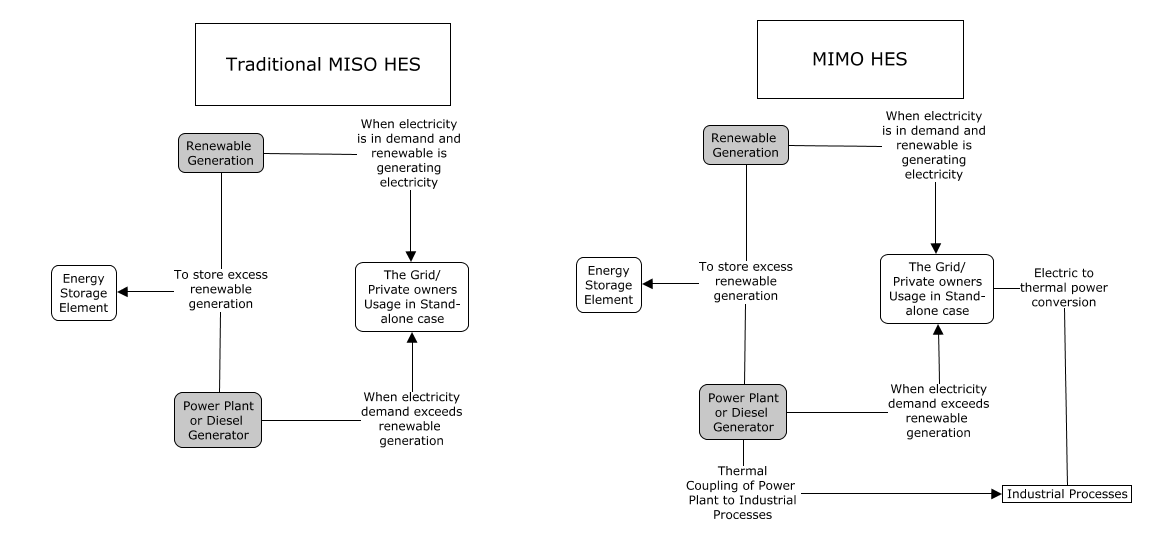
\includegraphics[width=\textwidth]{MISO_MIMO.png}
\caption{\small \sl This figure compares the MISO and MIMO configurations demonstrating the differences between traditional hybrid energy systems that are focused on generating reliable electricity and non-traditional hybrid energy systems which have the added objective of generating an additional product.  While many of the elements are the same, the MIMO system includes  Industrial Process which is either thermally or electrically coupled.}
\end{figure*}

\subsection{Nuclear Renewable Hybrid Energy Systems}

Nuclear Renewable Hybrid Energy Systems (NRHES) are defined by Bragg-Sitton et al. (2014) as the "tighter coupling of nuclear and renewable energy sources in a manner that better optimizes energy use for the combined electricity, industrial manufacturing, and transportation sectors capable of apportioning thermal electrical energy to first meet the grid demand (with appropriate power conversion systems), then utilizing excess thermal and, in some cases, electrical energy to drive a process that results in an additional product \cite {Bragg-Sitton2014}".  The potential benefit of co-locating the various facilities in the NRHES is optimizing the system to minimize cost to the NRHES as a whole while increasing economic resilience by diversifying both the means of generating energy as well as the products produced. For example, if natural gas prices increase, there could be less reliance on the natural gas plant and more focus on storage.  On a more short term perspective, if electricity prices are negative, the energy produced by the NRHES can be diverted to the industrial process. The drawbacks of co-locating the various generation sources and the industrial processes are the increased complexity of the system.  Furthermore, a nuclear power plant has never been thermally coupled in the United States at this point.  The low level state of development as well as the lack of experimental data suggest a lot of rigorous technical work needing to be developed.  There are regulatory concerns with a thermally coupled NRHES  

The additional products include, but are not limited to: synthetic fuel, titanium, desalinated water, hydrogen, aluminum, and heat pumps \cite{Bienvenue2015}. The NPP diverts the energy it generates between the grid and the industrial process to maximize profit. The system can allocate energy based on the market value of each of the multiple outputs produced. In the case of a NPP coupled with a desalination plant, for example, if the price of electricity is low, more thermal and/or electric energy can be diverted to generate more clean water at a higher profit \cite {Chen2016}. The costs of running a dynamic system, such as the case with a NRHES, include additional wear and tear, decreased thermal efficiency, and increased complexity of operations \cite{Garcia2013}. The total costs of the system, such as meeting regulatory expectations, have yet to be determined.

There have been no physical demonstrations to date of NRHES. Therefore, research has largely focused on computational modeling to determine the feasibility and optimization of coupling elements \cite{Boardman2013, Shropshire2012}. Creating a model for a NRHES is important for determining technical as well as economic optimization of the elements that could comprise such systems. Models are used as a means for forecasting limitations and functionality in specific conditions in order to ensure safety and reliable electricity production. Computational models can provide feedback regarding which NRHES models are worth pursuing given the expected profitability. A NRHES simulator could help inform policy and technology decisions on the bases of cost, flexibility, safety, and reliability. 

Our literature review revealed that a lot of work on NRHES is in the design and analysis stage \cite{Boardman2013, Shropshire2012}. Research is focused on developing a model that can dynamically simulate the contributions of variable energy sources, the constraints of fluctuating electricity demand, and thermal/electrical power demands for various industrial processes. The models focus on answering questions regarding minimizing the cost of electricity and ensuring profitability for each of the components comprising the NRHES. In order to move forward with development of any NRHES,  such systems must demonstrate that they can be profitable and can reliably respond to fluctuating electricity production and demand \cite{Rabiti2015}. 

An ongoing effort at Idaho National Laboratory (INL), Argonne National Laboratory (ANL), and Oak Ridge National Laboratory (ORNL) focuses on modeling a generic NRHES. The generic nature of the plant means that local variability in the costs of each of the components in the model is not taken into consideration. The generic model will test the economic viability of NRHES to determine if future development should be pursued. The industrial plant combines a nuclear power plant, a wind farm, a natural gas power plant, a battery, and a high temperature steam electrolysis hydrogen production facility. More component models will be developed in the future that can allow for the comparison of various industrial customers\cite{Harrison2016}. The chosen renewable source, a wind farm, models a highly stochastic system due to the unpredictable nature of wind generation \cite{Chen2016_wind}. The model optimizes the sizes of the nuclear power plant, the natural gas plant, and the battery. The objective is to choose the NRHES configuration that minimizes costs while meeting set emissions and grid reliability expectations.  


\subsection{Computational Tools}
NRHES sit in an interesting location in computational modeling. Many tools have been developed to model nuclear reactors and the nuclear fuel cycle as demonstrated in the nuclear fuel cycle simulators shown in Figure 2. Many tools have also been created to model and optimize non-nuclear hybrid energy systems (HOMER, Hybrid2, SOLSIM, SOMES, ARES, RAPSIM, HOGA)\cite {Bernal-Agustin2009}. These programs generate mass flow and calculate electricity output and the possible output of another product, such as hydrogen. Modelica and Excel, while neither specifically HES or NRHES tools, have been used to model both nuclear and non-nuclear hybrid energy systems \cite{Shropshire2012, Chen2016, Binder2014, Garcia2015, Epiney2016}. HES tools are typically bought for microgrid standalone systems. The main challenges to applying HES systems to a NRHES are the scale of the system being modeled and including the grid demand.

\section{NRHES Models}
There are criteria that make a tool better for modeling a NRHES. In order to select a tool to model a NRHES, it is necessary to understand what characteristics a model must possess in order to provide accurate information. For example, as discussed below, it is important for a NRHES model to incorporate the dynamic nature of the system in order to include losses from the fluctuations in the system. Understanding the differences among the underlying mathematical models as well as the software functionality is essential in determining whether and how a nuclear fuel cycle simulator (NFCS) will be useful to NRHES modeling . 
As mentioned above, the model currently under development by the Oak Ridge National Laboratory, the Argonne National Laboratory, and the Idaho National Laboratory has reviewed the essential characteristics for a computational model of NRHES. Rabiti et al. (2015) discusses the important elements of a NRHES computational model in detail, describing the basic requirements of the software as a "computational representation of the thermal, mechanical, chemical, and electrical processes in the systems as process units, reactors, manufacturing plants, and energy delivery (to the appropriate point of interface with the market transaction, such as an electricity bus, or a product depot or distribution terminal where a commodity price is established)"\cite{Rabiti2015}. The model in development by the national laboratories combines RAVEN (Reactor Analysis and Virtual Control Environment) for the stochastic aspects of the system and Modelica for modeling the various components in the NRHES. 

\subsection{RAVEN}
The RAVEN tool was initially built for probabilistic risk assessment. RAVEN, as a probabilistic tool, is "able to perform parametric and stochastic analysis based on the response of complex system codes\cite{RabitiRAVEN}." RAVEN is used to run thousands of different wind energy generation paths in order to generate a statistically fair representation of how renewables, in this case wind power, would likely function over any given hour. RAVEN can be used to generate the most generic seasonal wind generation over a week. The model can be tailored to specific regions, defining the costs of inputs such as water and natural gas based on the typical regional price, as well as selling the electricity for the current regional rate. A typical week can be extrapolated to represent a given season. The process can be repeated over the different seasons, which can be extrapolated to represent however long of a time frame is desired to run the NRHES simulation. Using synthetic generated data instead of historic data avoids the critique that the model only represents past behavior and is thus inapplicable to future trends \cite{redfoot_epiney_2016}. RAVEN is also used to determine high-risk time series samples to ensure that high risk scenarios are accounted for in the study. Since both the loss of load probability and the sensitivity to uncertainty analysis rely on probabilistic assessment, RAVEN also calculates these figures of merit. 

\subsection{Dynamic Modeling}
In Garcia et. al. (2013) and Du et. al. (2014), a dynamic approach to modeling hybrid energy systems (HES) is applied in order to appropriately address the impacts of flexible operation of the system due to variable renewable generation \cite{Garcia2013, Du2014}. In Du et. al. (2014), two optimization problems are addressed: the first minimizes variability in the HES through optimizing components of the HES system, and the second imposes operating and capital costs on the design variables. Garcia et. al. (2013) has a two-part series. The first applies and analyzes performance of a dynamic approach to modeling some of the physical components of a traditional and an advanced (produces goods besides electricity) HES. The second paper focuses on economic effects using a dynamic approach, as opposed to time series or statistical analysis. Overall, both parts of the series focus on how a dynamic approach better models the high level of variability of a HES for output generation and profitability maximization \cite{Garcia2013}. The costs of operating in a flexible manner, dynamically allocating resources between multiple coupled systems, are substantial enough to require a simulation that precisely models the variability of the system \cite{Garcia2013, Shropshire2011, Locatelli2015}. The dynamic modeling at this point focuses on the dynamic transfer of energy to different sources, and how this impacts the economics and grid reliability. The physical impacts of the grid system have not yet been included in the model \cite{Harrison2016}.  The dynamic allocation of the heat and electricity depending on the renewable generation and the grid demand is an essential characteristics of an NRHES.  Including factors such as how quickly the NRHES will be able to switch between providing energy to the industrial facility and the grid will impact determining whether a NRHES is worth pursuing. 

\subsection{Modelica}
Modelica is a widely used open source language for modeling large and complex systems composed of smaller component models. It is particularly optimized for modeling dynamic systems. Modelica has powerful libraries, such as Thermopower, that include the thermohydraulic modeling tools required for modeling mass flows in energy systems \cite{Binder2014}. The language is well-maintained, giving it the added benefits of having up-to-date documentation and a community that can provide support. Typically Modelica is run on the Dymola developer environment, a private tool developed by the creator of Modelica, Dr. Hilding Elmquist. Another option for running the Modelica language is the open source OpenModelica environment.

A Modelica HES model developed in Binder et. al. (2014) includes a nuclear reactor, two steam cycles, a chemical plant, and an electrical component \cite{Binder2014}. The products of this Modelica NRHES model are synthetic fuel and electricity. The model includes the ramp up stage when the reactor initially starts or is increasing from a lower load. The steam generator connected to the NPP determines which of its turbines to use depending on electricity demand, the 60\% turbine, the 30\% turbine, or the 15\% turbine, which can be used in unison. A pressure relief valve releases excess energy unused by the turbines. The wind generation is modeled using the Western Wind dataset from the National Renewable Energy Laboratory (NREL) for an unspecified region in Idaho. Each component in the model was tested individually before being combined. Using the individual component models, verifications were made for the system as a whole. The startup transient state of the model took much greater computation time due to the complex interrelations of the components. Generally, to run a model of a NRHES, including using Modelica, requires a control algorithm, a differential equation that controls how the dynamic system allocates heat. The profitability control algorithm can be adjusted to incorporate varying parameters such as the price of electricity or the cost of natural gas. The study concluded that Modelica, due to its ability to evaluate control algorithms, is an effective tool for dynamically modeling a HES.

\subsection{Small Modular Reactors}
For completeness, we will address the use of small modular reactors as both tools for load following and sources of process heat. Locatelli (2015) discusses the technical and economic feasibility of load following using multiple small modular reactors (SMRs), applying the excess energy toward generating algae-biofuel and desalinated water \cite{Locatelli2015}. SMRs are generally defined as nuclear reactors under 300 MWe. They can be combined to meet the demanded energy output. SMRs are a promising possibility for NRHES due to their ability to add additional modules as electricity demand in a given region increases. Multiple SMRs have a clear means of load following, simply by shutting down those reactors whose energy output is not required due to seasonal shifts etc. This same modularity allows the energy produced from a given SMR to be diverted to an industrial process, while others are conscripted for electricity output. The modularity of the SMRs allows greater flexibility in the design of the industrial park.  Locatelli et. al. discusses the benefits as well as drawbacks of an NRHES that includes a thermal desalination process~\cite {Locatelli2015}. A desalination plant has the benefits of switching between a latent and producing state and generating a product that is readily stored. The main drawback is poor water quality and output level for when the desalination unit is restarted.

\subsection{Other Research on NRHES Models}
Many more studies on HES and NRHES incorporate economic and technical modeling, but the essential characteristics of ability to model a dynamic and stochastic system have been covered. Some other relevant studies include: 
\begin{itemize}
\item Shropshire et. al. (2012) does not focus on HES, but discusses how different models of flexible and small modular reactors could integrate into the European energy market with growing renewable generation, thus fulfilling the growing need for flexibility and load following in other electricity suppliers \cite{Shropshire2012}. 
\item Shropshire et. al. (2011) developed target cost estimates for reactors given certain economic environments based on competing technology energy costs \cite{Shropshire2011}. 
\item NEA-OECD (2011) presents an overview of the capability of implemented newer and older nuclear power plants to load follow \cite{Nuclear2011}. 
\item Baker (2016) applies the levelized cost of electricity (LCOE) as the figure-of-merit (FOM) and the role of battery storage to evaluate different NRHES scenarios \cite{Baker2016}
\item Kazimi et al. (2009) does a preliminary dynamic analysis of two NRHES systems that have high levels of renewable energy generation and multiple outputs from the system. The study concluded that NRHES could lead to optimized energy use, reduced carbon, favorable economic performance, and flexible operation time \cite{Kazimi}. 
\item Forsberg et. al. (2009) discusses using nuclear power to create more liquid transportation fuels from biomass and fossil fuel sources \cite{Forsberg2009}. 
\item There have also been two regional modeling studies done on Texas and Arizona focused on including regional characteristics to determine the renewable used and the industrial process.  
\end{itemize}

Table I displays the characteristics routinely described as necessary to model a NRHES along with their citations.

\begin{table}[h!]
\centering
\caption{References for Each NRHES Characteristic}
\begin{tabular}{ ||c | c|| }
 \hline 
 NHES Characteristic & Paper \\ [0.5ex]
 \hline \hline
 Dynamic & \cite{Garcia2013, Du2014, Kazimi, Garcia2016}\\
 \hline
 Sensitivity Analysis & \cite{Shropshire2011, Rehman2010, Adaramola2014, Chen2016}\\
 \hline
 Optimization of components & \cite{Chen2016,Ozcan2016, Forsberg2009,Garcia2015,Aumeier2011}\\
 \hline
 Stochastic Model of Renewables & \cite{Rabiti2015, Garcia2016,Locatelli2015}\\ 
 \hline
 Grid Demand model & \cite{Forsberg2013, Garcia2016,Garcia2013,Ruth2014,Chen2016}\\
 \hline
  Economic FOMs & \cite{Garcia2016,Chen2016,Rabiti2015,Epiney2016,Bragg-Sitton2014}\\
 \hline
\end{tabular}
\label{table:1}
\end{table}

The table displays the characteristics that arise as a pattern in many of the documents.  The six characteristics likely need to be included in a NRHES model.  Each of these characteristics have been included in previous studies, and thus have some already proposed approaches.  The characteristics can be studied in greater detail in order to determine if they satisfactorily model the system. A NFCS would need to find a way to appropriately include these characteristics.

\section{Nuclear Fuel Cycle Simulators}

The common uranium nuclear fuel cycle describes the system of mining uranium, converting the uranium to gaseous UF6, enriching the uranium with higher percentages of U235, fabricating the fuel, the fuel changing in the reactor, storage, reprocessing, and final disposal. There are different fuel cycles, depending on the type of reactor used and how the spent fuel coming out of the reactor is treated. Nuclear fuel cycle simulators model the fuel cycle determining the likely quantity and characteristics of nuclear fuel generally in order to determine future policies surrounding management of the spent fuel. 
  
This section identifies basic properties of nuclear fuel cycle simulators and assesses their distinct functionality. Figures 2a and 2b display many of the currently used nuclear fuel cycle simulators (NFCS). The fuel cycle simulators are the central nodes in these figures, with the tools for computing some of the basic descriptive qualities of a fuel cycle branching off. The computational attributes that are often included in NFCS are: mass flows, reactor physics, thermal hydraulics, reprocessing, waste management, risk management, and economics. While different fuel cycle simulators were initially optimized for a variety of applications, there is a lot of overlap in their functionality \cite {Guerin2009}. Because nuclear fuel cycle simulators are attempting to model the same thing, the nuclear fuel cycle, the models include some means of tracking the fuels as they move through the fuel cycle and a means of tracking the composition of the fuel. The different fuel cycle simulators generally have the ability to simulate fleets of nuclear reactors with the associated fuel cycle industrial processes and nuclear materials storage. As can be seen in figues 2a and 2b, there are a good number of NFCS which all have different functionality and dependencies.  There is a degree of complexity in determining which NFCS best fits the research objective.

\begin{subfigures}
\begin{figure*}
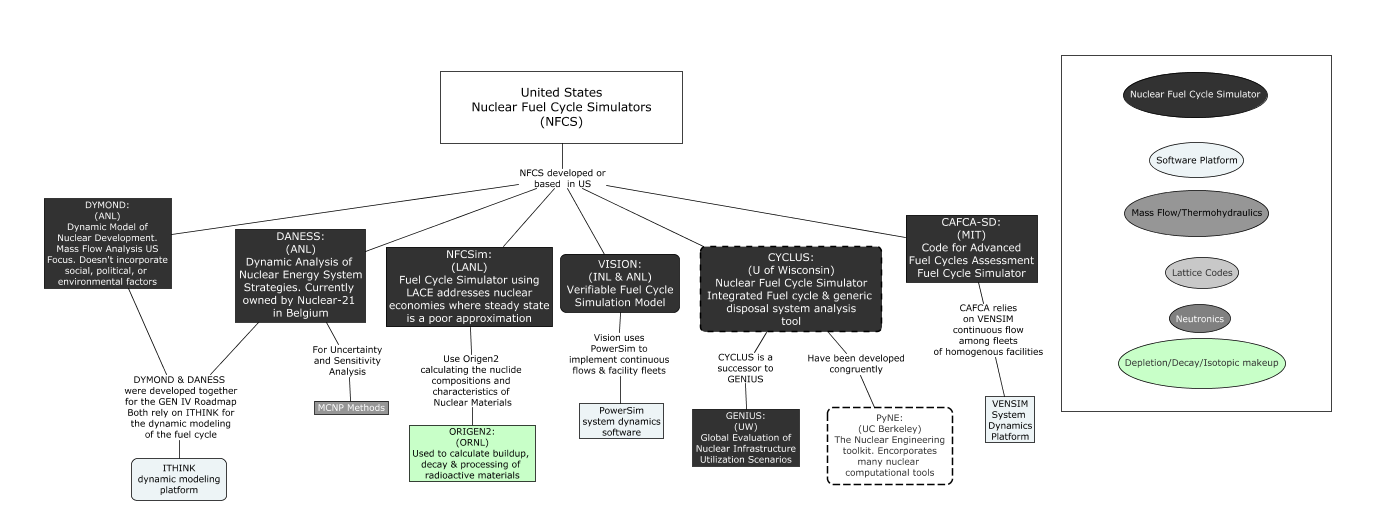
\includegraphics[width=\textwidth]{US_FUEL_TOOLS.png}
\caption{\small \sl This figure displays the nuclear fuel cycle simulators developed in the United States, though they are not necessarily specifically built to demonstrate the development of a US fuel cycle. This figure does not include all nuclear fuel cycle simulators or their dependencies.  The figure demonstrates some of the complexity of the current Nuclear Fuel Cycle Simulator options. The figure demonstrates the types of tools NFCSs depend on, thereby suggesting some of their functionality.}
\end{figure*}

\begin{figure*}
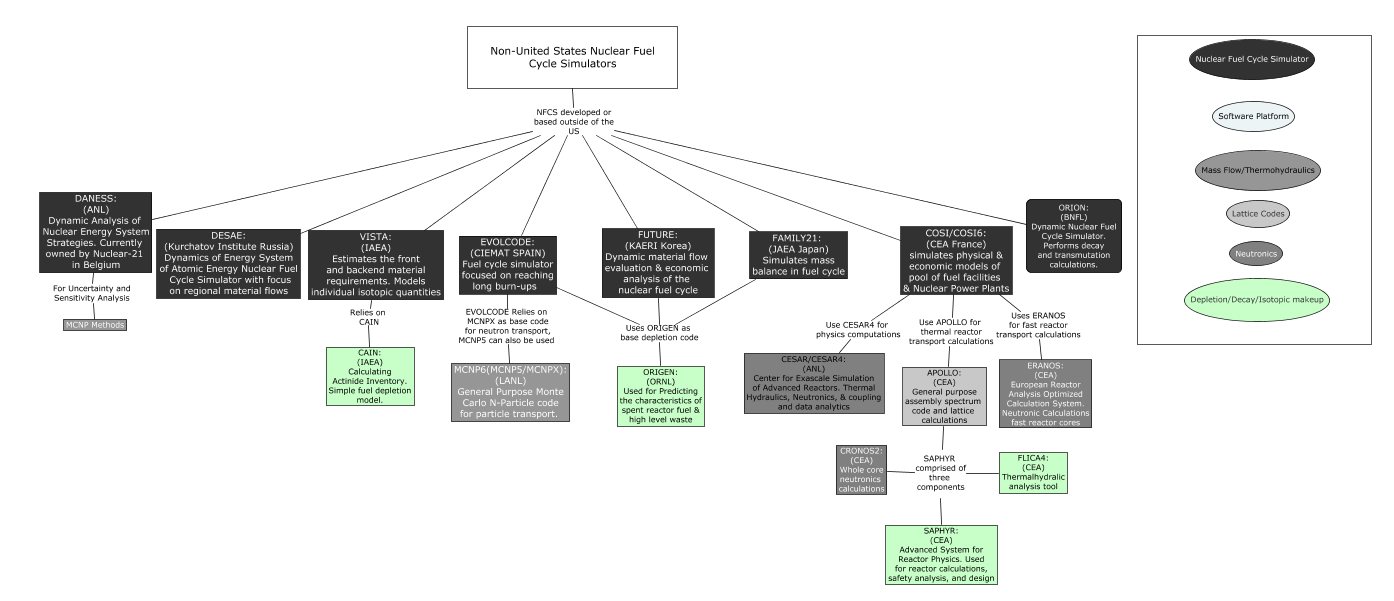
\includegraphics[width=\textwidth]{Non-US_FUEL_TOOLS.png}
\caption{\small \sl This figure displays the nuclear fuel cycle simulators developed outside of the United States.The full relationship between the various computational tools may not be covered.  The literature is lacking in descriptions of the evolution and dependencies of the computational tools.}
\end{figure*}
\end{subfigures}

The assumed fuel cycle for the NRHES model currently being built is the once-through fuel cycle, or when the nuclear fuel is used once in a nuclear reactor then sent to long term disposal. In the case of the once-through fuel cycle, uranium is mined, enriched for a higher concentration of U-235, molded into fuel assemblies, and used in a nuclear reactor for between 36 and 72 months. The spent fuel is not reprocessed, so it is first stored in spent fuel pools, then canisters, both onsite, and eventually will be disposed of in a deep geologic repository. More advanced fuel cycles involve different degrees and methods of used fuel reprocessing. Nuclear fuel cycle simulators permit modeling of new techniques applied to all parts of the nuclear fuel cycle; from the mining through the waste management. The idea behind modeling the full nuclear fuel cycle is to optimize the fuel cycle given technical, environmental, political, and economic constraints.

The Prof. Paul P. H. Wilson report for the Blue Ribbon Commission on America’s Nuclear Future "Comparing Nuclear Fuel Cycle Options" discusses, at a high level, different nuclear fuel cycle simulators' performance for a once-through system, a limited recycling option, as well as continuous recycling. Prof. Wilson describes nuclear fuel cycle simulators as focusing "on understanding mass flows and facility deployments under alternative civilian nuclear fuel cycles, particularly during transitions between fuel cycles." The two uses for a NFCS as stated in the report are to make informed policy decisions and to determine more fine-grained technical decisions about what technologies to pursue. Prof. Wilson breaks down some of the assumptions either explicitly or implicitly stated in the nuclear fuel cycle simulators, including:
\begin{itemize}
\item "Growth rate of nuclear electricity, 
\item Date of introduction of new technologies and facilities, 
\item Constraints on spent fuel interim storage capacity, 
\item Constraints on spent fuel storage/cooling times,
\item Constraints on quantity of separated plutonium, 
\item Relative priority of different fuel cycle paths, and 
\item Supply vs. demand flow control at each fuel cycle stage."
\end{itemize}

Prof. Wilson explains that there is also a degree of uncertainty present in each of the assumptions, introducing even greater variability. NFCS differ both in how they calculate their FOMs as well as in how the FOMs are presented. Benchmarks for NFCSs often entail summaries for each fuel cycle simulator by the authors of the tool \cite{Guerin2009}. Making comparisons of various tools is difficult since we must rely on the reports of the developers rather than using controlled end user. Different authors choose to discuss different aspects of the NFCS, adding to the difficulty of comparing the various NFCS. Even when two NFCSs have similar functionality, it can be hard to make comparisons based on benchmark reports due to different emphases in the reports describing the tools. This leads to model development with built-in biases that weigh certain characteristics of a technology as more important, thereby skewing the results. 

Due to the uncertainties, NFCSs are best used as comparative tools, as opposed to predicting absolute values. Given different constraints within an NFCS, it can demonstrate the relative differences between the two simulations better than the absolute nature of either one. The strength of relative comparisons is especially true in economic analyses, where the true prices and how they are likely to change over time are unpredictable. The simulator, if built well, would be able to show which model would be cheaper, not the exact price associated with it  \cite{Wilson2012}. Some of the uncertainty concerns surrounding simulating a nuclear fuel cycle as stated by Prof. Wilson:

\begin{itemize}
\item Cost of water
\item Uranium consumption and costs
\item Total land use
\item Waste disposal space
\item Localized variations of the estimated peak dose rate
\item Radiotoxicity of waste streams
\item Radioactive liquid and gaseous release volumes
\item Conventional pollutant release over the lifecycle of the nuclear system
\item Required Enrichment of the fuel
\item Attractiveness of separated materials for proliferation of nuclear weapons
\item Difficulties in siting a nuclear power plant, and
\item Variation in how metrics are calculated.
\end{itemize}

Many of the above listed characteristics are region specific capital and operations and maintenance costs that would also apply to NRHES.  In order to include these characteristics for both the nuclear fuel cycle and NRHES, some measures of uncertainty would need to account for the variability of circumstances. Wilson breaks down the uncertainties into the categories of cost, safety, resource utilization, sustainability, and non-proliferation ~\cite {Wilson2012}. 

The major difference between many of these nuclear fuel cycle simulators is the ability to model discrete facilities and fuel batches versus modeling continuous mass flows throughout the fleet of facilities operating in an identical fashion. In the case of the fleet modeling, the average value for each of the facilities is assumed. The discrete model requires more information while providing a more detailed analysis. The discrete model is, however, more computationally complex and expensive.

In "Modeling the Nuclear Fuel Cycle," Juchau et al. (2010) describe four functions as necessary for a NFCS to meet the desired qualities of an organization proposed at the time called the Simulation Institute for Nuclear Enterprise Modeling and Analysis \cite{Juchau2010}. The four functions, which reiterate the characteristics described by Prof. Wilson, include:

\begin{itemize}
\item "Characterize and deploy individual fuel cycle facilities and reactors in a simulation while discretely tracking material movements,
\item The capability to perform an uncertainty analysis for each element of the fuel cycle and an aggregate uncertainty analysis,
\item Inclusion of an optimization engine able to optimize simultaneously across multiple objective functions, and 
\item Open and accessible code software and documentation to aid in collaboration between multiple entities and to facilitate software updates." 
\end{itemize}

Juchau (2010) reviews the nuclear fuel cycle simulator tools CAFCA, COSI, CEPMNFC, DANESS, NFCSim, VEGAS, VISION, NFCSS, and GENIUS 1. His conclusion is that many of these tools have overlapping functionalities, partially due to the proprietary nature of at least parts of each. One of the reasons why there are so many nuclear fuel cycle simulators is that many of the countries that currently have NPPs have designed their own simulators. Figure 3 depicts the non-US NFCSs along with some of their software dependencies. Most of the fuel cycle simulators are not open source or available for download; thus, each nation tends to have proprietary software. As discussed with Prof. Kathryn D. Huff, it is also often more efficient, both in terms of time spent as well as better integration, if the different functions are designed by the same team (\cite{redfoot_huff_2016}). Integrating components, such a burnup calculation, from one system into a new system can often be more challenging than building the function from scratch. While sharing code can be challenging amongst various program, some calculations or libraries are commonly used by NFCSs. For example, Figure 3 depicts EVOLCODE, FUTURE, and FAMILY21 as all relying on Origen.

\section{Analysis}
The underlying structure of passing materials between various facilities is similar enough between nuclear materials in a fuel cycle and heat or electricity flow in a nuclear hybrid energy system that a nuclear fuel cycle simulator could model a nuclear renewable hybrid energy system. In the case of a NRHES model, the facilities are the NPP, the renewable, and the industrial process at least.  In the case of the nuclear fuel cycle, the facilities are the steps in the given fuel cycle. Both systems are time dependent and include uncertainty measures. Many of the uncertainty measures found in NFCS are the same for NRHES including O\&M costs, water costs, and challenges in siting a nuclear power plant. Optimally, both systems would be: 
\begin{itemize}

\item flexible so that new component models and specific regional characteristics could easily be added, 
\item open source so that researchers can use the tools instead of rebuilding already available tools, and 
\item usable by technical and non technical people alike to address policy decisions. 

\end{itemize}
 
A NFCS would need to be able to reasonably model the dynamic nature of NRHES. The dynamics aspects of concern, at this point in the research, are how the energy would switch between different loads as well as the ramping of various generation components.  The nuclear fuel cycle does not require the quantities to be exchanged nearly as regularly as a nuclear hybrid energy system and with as inconsistent of quantities. The dynamic impacts on the physical system would need to be included in order to generate a meaningful model of a NRHES. The stochastic aspect of the renewables components of a NRHES would also require either external coupling with a tool able to model randomness such as RAVEN or the use of real time data from a specific region. The dynamic and stochastic components of modeling a nuclear hybrid energy system would take some work to incorporate. 

Many of the features commonly found in a NFCS would not be needed in a NRHES model.  There would be no need to model a fleet of NRHES at this point in development, so a system would have to be able to model discreet facilities.  The reactor calculations, such as burnup, would not be needed for a NRHES.  The back end of the fuel cycle, such as models for reprocessing and long term waste storage would also not be applicable at this point to a NRHES model.  The primary qualities that would be used are optimization methods, economic evaluation, and means of exchanging materials in a system.  


\section{CYCLUS and Future Research}

As CYCLUS is the only nuclear fuel cycle simulator that has the benefits of being both open source and built in a modern programming language, it is the NFCS worth pursuing to model NRHES. The flexibility and modular design of CYCLUS suggest the potential of CYCLUS successfully modeling a NRHES. The CYCLUS fuel cycle simulator's primary tool is the dynamic resource exchange (DRE) \cite{Huff2016}.  The DRE has a set time step at which point certain facilities will put their resource up on the market for exchange while other facilities can make a bid for a certain amount of the resource. For example, in the case of modeling the nuclear fuel cycle, the reactor could declare how much spent fuel it has once every eighteen months.  A reprocessing facility and a long term geologic repository could both bid on how much of the spent fuel each facility could take at that point.  The DRE has a built in functionality of preferences for allocating a resource.  For the example given, there could be a built in preference for the reprocessing facility, meeting the bid from this facility before sending the remaining spent fuel resource to the long term geologic repository. The simulation could be run over hundreds of years to demonstrate the accumulation of spent fuel and fission products over the given time line. 

The DRE tool is sufficiently flexible to model other resources besides nuclear fuel, due to the ability to build new archetypes which do not include nuclear fuel specific characteristics.  In the case of a NRHES, the DRE would be passing the electricity or heat to the various facilities.  The reactor would thus, at a time step of 1 minute for example, pass heat to the industrial process and electricity to the grid.  The renewable would pass electricity to the grid when generating.  The grid would make a bid every minute for how much electricity is demanded.  The industrial process would also make a bid for the heat and/or electricity required.  The built in preferences functionality in CYCLUS could be used to ensure the resource is sent to the facility willing to pay the highest price for the resource.  Thus, the electricity or heat could be sent to the industrial process when the product created with that energy is worth more than the current value of electricity on the grid.
% * <eredfoot@gmail.com> 2017-08-28T17:18:25.734Z:
% 
% > The DRE tool
% Practice comment
% 
% ^ <eredfoot@gmail.com> 2017-08-28T18:09:27.966Z.

While there are some interesting potential benefits to a NRHES, such as diversifying sources of electricity production, co-locating the facilities have some potential drawbacks.  Integrating exclusively through the grid results in a decoupling of potentially negative feedback effects \cite{Harrison2016}.  A meaningful model would be able to compare a NRHES to the current grid system. The CYCLUS tool could be used to model the difference between co-locating the given facilities in a NRHES as compared to each of the facilities acting independently at different nodes on the grid.  The DRE could track the profitability of each of the facilities independently, each of the generation sources selling electricity to the grid and the industrial facility producing a product.  The DRE could also treat the system as a single facility that outputs two products, the industrial good and electricity to the grid. Along with profitability, other important figures of merit, such as emissions and hours not meeting the grid demand could be tracked and compared in CYCLUS. 

Future research will focus on using CYCLUS as a deployment tool for electricity \cite{redfoot_rabiti_2017}. The DRE would be able to put some quantity of heat or electricity on the resource exchange market.  The industrial process or grid could each bid for the heat using economics or other preference model.  The time step for the DRE would be very short, on the order of a minute, in order for the model to output valuable information. 

From the literature review on NRHES, a notable gap in the current modeling research is the benefits gained from thermally coupling systems as compared to electrically coupling.  The efficiency and conversion benefits would have to be greater than the costs associated with co-location.  CYCLUS's ability to dispatch resources could allow for a comparison between coupling an industrial process thermally or electrically. CYCLUS would be used to compare a system that exclusively produces electricity, but varies in the amount of electricity sent to the industrial process, with a system which sends process heat directly from the reactor to the industrial process as well as sending electricity to the grid.   New archetypes for the waste heat could also be included in order to determine if uses for waste heat are worth pursuing.  Future research will focus on building the archetypes for allocating the heat and electricity in a NRHES.  

\section{Summary Remarks}
The nuclear fuel cycle shares similar enough underlying characteristics to a nuclear hybrid energy system to loosely model the system. The major challenge in modeling a NRHES with a NFCS is including the dynamic aspects of the system and how that will affect the overall costs of the system. A NFCS that is in a mature state of development, open source, easy to incorporate new components, flexible enough to change the materials exchanged rapidly, and able to be coupled with external tools for modeling the renewable resource could speed up the development of a NRHES model. CYCLUS is the only currently open source nuclear fuel cycle simulator.  As such, CYCLUS makes the most sense of the NFCSs to pursue in developing an NRHES.
\end{linenumbers}

%%%%%%%%%%%%%%%%%%%%%%%%%%%%%%%%%%%%%%%%%%%%%%%%%%%%%%%%%%%%%%%%%%%%%%%%%%%%%%%%

\pagebreak
\section*{Acknowledgments}

Thank you to Dr. Shannon Bragg-Sitton, Dr. Cristian Rabiti, Dr. Aaron Epiney, Dr. Jong Suk Kim, and Dr. Kathryn Huff for their time and insight.  

\pagebreak
\bibliographystyle{ans_js}                                                                           %custom ANS journal submission template bibliography style
\bibliography{bibliography}

%%% If you desire to place footnotes at the end of the document, uncomment these two lines and the four related near the beginning of this file
%\pagebreak
%\theendnotes

\end{document}


